\chapter{哈密顿图}
\begin{Ex}
  以下4个图中,存在一个哈密顿圈的是$\underline{\quad\quad}$。
  \vspace{0.5cm}

  A.
    \begin{minipage}{0.18\linewidth}
    \centering
    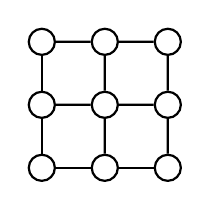
\begin{tikzpicture}[auto,
    specification/.style ={circle, draw, thick}, scale = 0.8]
   \node[specification] (A)  at (0,0)  {};
   \node[specification] (B)  at (1,0)  {};
   \node[specification] (C)  at (2,0)  {};
   \node[specification] (D)  at (0,1)  {};
   \node[specification] (E)  at (1,1)  {};
   \node[specification] (F)  at (2,1)  {};
   \node[specification] (G)  at (0,2)  {};
   \node[specification] (H)  at (1,2)  {};
   \node[specification] (I)  at (2,2)  {};

   \draw[thick] (A) to  (B);
   \draw[thick] (B) to  (C);
   \draw[thick] (D) to  (E);
   \draw[thick] (E) to  (F);
   \draw[thick] (G) to (H);
   \draw[thick] (H) to (I);
   \draw[thick] (A) to (D);
   \draw[thick] (B) to (E);
   \draw[thick] (C) to (F);
   \draw[thick] (D) to (G);
   \draw[thick] (E) to (H);
   \draw[thick] (F) to (I);
 \end{tikzpicture}
\end{minipage}\hfill
  B.
    \begin{minipage}{0.18\linewidth}
    \centering
    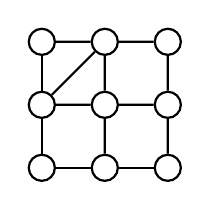
\begin{tikzpicture}[auto,
    specification/.style ={circle, draw, thick}, scale = 0.8]
   \node[specification] (A)  at (0,0)  {};
   \node[specification] (B)  at (1,0)  {};
   \node[specification] (C)  at (2,0)  {};
   \node[specification] (D)  at (0,1)  {};
   \node[specification] (E)  at (1,1)  {};
   \node[specification] (F)  at (2,1)  {};
   \node[specification] (G)  at (0,2)  {};
   \node[specification] (H)  at (1,2)  {};
   \node[specification] (I)  at (2,2)  {};

   \draw[thick] (A) to  (B);
   \draw[thick] (B) to  (C);
   \draw[thick] (D) to  (E);
   \draw[thick] (E) to  (F);
   \draw[thick] (G) to (H);
   \draw[thick] (H) to (I);
   \draw[thick] (A) to (D);
   \draw[thick] (B) to (E);
   \draw[thick] (C) to (F);
   \draw[thick] (D) to (G);
   \draw[thick] (E) to (H);
   \draw[thick] (F) to (I);
   \draw[thick] (D) to (H);

 \end{tikzpicture}
\end{minipage}\hfill
      C.
    \begin{minipage}{0.18\linewidth}
    \centering
    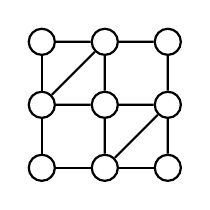
\begin{tikzpicture}[auto,
    specification/.style ={circle, draw, thick}, scale=0.8]
   \node[specification] (A)  at (0,0)  {};
   \node[specification] (B)  at (1,0)  {};
   \node[specification] (C)  at (2,0)  {};
   \node[specification] (D)  at (0,1)  {};
   \node[specification] (E)  at (1,1)  {};
   \node[specification] (F)  at (2,1)  {};
   \node[specification] (G)  at (0,2)  {};
   \node[specification] (H)  at (1,2)  {};
   \node[specification] (I)  at (2,2)  {};

   \draw[thick] (A) to  (B);
   \draw[thick] (B) to  (C);
   \draw[thick] (D) to  (E);
   \draw[thick] (E) to  (F);
   \draw[thick] (G) to (H);
   \draw[thick] (H) to (I);
   \draw[thick] (A) to (D);
   \draw[thick] (B) to (E);
   \draw[thick] (C) to (F);
   \draw[thick] (D) to (G);
   \draw[thick] (E) to (H);
   \draw[thick] (F) to (I);
   \draw[thick] (D) to (H);
   \draw[thick] (B) to (F);
 \end{tikzpicture}
\end{minipage}\hfill
      D.
    \begin{minipage}{0.18\linewidth}
    \centering
    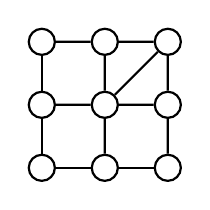
\begin{tikzpicture}[auto,
    specification/.style ={circle, draw, thick}, scale=0.8]
   \node[specification] (A)  at (0,0)  {};
   \node[specification] (B)  at (1,0)  {};
   \node[specification] (C)  at (2,0)  {};
   \node[specification] (D)  at (0,1)  {};
   \node[specification] (E)  at (1,1)  {};
   \node[specification] (F)  at (2,1)  {};
   \node[specification] (G)  at (0,2)  {};
   \node[specification] (H)  at (1,2)  {};
   \node[specification] (I)  at (2,2)  {};

   \draw[thick] (A) to  (B);
   \draw[thick] (B) to  (C);
   \draw[thick] (D) to  (E);
   \draw[thick] (E) to  (F);
   \draw[thick] (G) to (H);
   \draw[thick] (H) to (I);
   \draw[thick] (A) to (D);
   \draw[thick] (B) to (E);
   \draw[thick] (C) to (F);
   \draw[thick] (D) to (G);
   \draw[thick] (E) to (H);
   \draw[thick] (F) to (I);
   \draw[thick] (E) to (I);

 \end{tikzpicture}
\end{minipage}\hfill

\end{Ex}

\begin{Ex}
  以下4个图中,不存在哈密顿路的是$\underline{\quad\quad}$。
  \vspace{0.5cm}

  A.
    \begin{minipage}{0.18\linewidth}
    \centering
    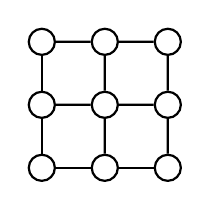
\begin{tikzpicture}[auto,
    specification/.style ={circle, draw, thick}, scale = 0.8]
   \node[specification] (A)  at (0,0)  {};
   \node[specification] (B)  at (1,0)  {};
   \node[specification] (C)  at (2,0)  {};
   \node[specification] (D)  at (0,1)  {};
   \node[specification] (E)  at (1,1)  {};
   \node[specification] (F)  at (2,1)  {};
   \node[specification] (G)  at (0,2)  {};
   \node[specification] (H)  at (1,2)  {};
   \node[specification] (I)  at (2,2)  {};

   \draw[thick] (A) to  (B);
   \draw[thick] (B) to  (C);
   \draw[thick] (D) to  (E);
   \draw[thick] (E) to  (F);
   \draw[thick] (G) to (H);
   \draw[thick] (H) to (I);
   \draw[thick] (A) to (D);
   \draw[thick] (B) to (E);
   \draw[thick] (C) to (F);
   \draw[thick] (D) to (G);
   \draw[thick] (E) to (H);
   \draw[thick] (F) to (I);
 \end{tikzpicture}
\end{minipage}\hfill
  B.
    \begin{minipage}{0.18\linewidth}
    \centering
    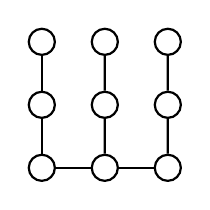
\begin{tikzpicture}[auto,
    specification/.style ={circle, draw, thick}, scale = 0.8]
   \node[specification] (A)  at (0,0)  {};
   \node[specification] (B)  at (1,0)  {};
   \node[specification] (C)  at (2,0)  {};
   \node[specification] (D)  at (0,1)  {};
   \node[specification] (E)  at (1,1)  {};
   \node[specification] (F)  at (2,1)  {};
   \node[specification] (G)  at (0,2)  {};
   \node[specification] (H)  at (1,2)  {};
   \node[specification] (I)  at (2,2)  {};

   \draw[thick] (A) to  (B);
   \draw[thick] (B) to  (C);
   \draw[thick] (A) to (D);
   \draw[thick] (B) to (E);
   \draw[thick] (C) to (F);
   \draw[thick] (D) to (G);
   \draw[thick] (E) to (H);
   \draw[thick] (F) to (I);

 \end{tikzpicture}
\end{minipage}\hfill
      C.
    \begin{minipage}{0.18\linewidth}
    \centering
    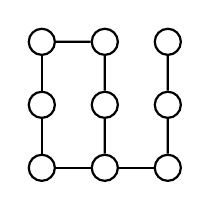
\begin{tikzpicture}[auto,
    specification/.style ={circle, draw, thick}, scale=0.8]
   \node[specification] (A)  at (0,0)  {};
   \node[specification] (B)  at (1,0)  {};
   \node[specification] (C)  at (2,0)  {};
   \node[specification] (D)  at (0,1)  {};
   \node[specification] (E)  at (1,1)  {};
   \node[specification] (F)  at (2,1)  {};
   \node[specification] (G)  at (0,2)  {};
   \node[specification] (H)  at (1,2)  {};
   \node[specification] (I)  at (2,2)  {};

   \draw[thick] (A) to  (B);
   \draw[thick] (B) to  (C);
   \draw[thick] (A) to (D);
   \draw[thick] (B) to (E);
   \draw[thick] (C) to (F);
   \draw[thick] (D) to (G);
   \draw[thick] (E) to (H);
   \draw[thick] (F) to (I);
   \draw[thick] (G) to (H);
 \end{tikzpicture}
\end{minipage}\hfill
      D.
    \begin{minipage}{0.18\linewidth}
    \centering
    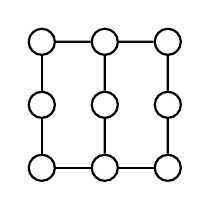
\begin{tikzpicture}[auto,
    specification/.style ={circle, draw, thick}, scale=0.8]
   \node[specification] (A)  at (0,0)  {};
   \node[specification] (B)  at (1,0)  {};
   \node[specification] (C)  at (2,0)  {};
   \node[specification] (D)  at (0,1)  {};
   \node[specification] (E)  at (1,1)  {};
   \node[specification] (F)  at (2,1)  {};
   \node[specification] (G)  at (0,2)  {};
   \node[specification] (H)  at (1,2)  {};
   \node[specification] (I)  at (2,2)  {};

      \draw[thick] (A) to  (B);
   \draw[thick] (B) to  (C);
   \draw[thick] (A) to (D);
   \draw[thick] (B) to (E);
   \draw[thick] (C) to (F);
   \draw[thick] (D) to (G);
   \draw[thick] (E) to (H);
   \draw[thick] (F) to (I);
   \draw[thick] (G) to (H);
   \draw[thick] (H) to (I);

 \end{tikzpicture}
\end{minipage}\hfill

\end{Ex}

